\documentclass[11pt]{article}
\usepackage[margin=2cm]{geometry}
\usepackage{polyglossia}
\setmainlanguage{french}
\usepackage{ltablex}
\usepackage{graphicx}
\usepackage{lscape}
\title{Compte Rendu TPCpp3}
\author{Benoit {\sc Renault}, Clément {\sc Espeute}}
\date{Décembre 2015}


\begin{document}

\maketitle

\section{Introduction}
Le programme \texttt{analog} permet de lire et d'extraire certaines informations intéressantes d'un fichier de log apache. Il permet entre autre de faire la liste des documents les plus consultés sur le serveur et d'établir un graphe des liens entre les différentes pages du site et de l'Internet et combien de fois ceux-ci ont été suivis. Le programme gère différents paramètres permettant par exemple d'ignorer certains types de fichiers ou de ne prendre en compte que les requêtes qui ont eu lieu à une heure donnée. 
\section{Spécifications}


\begin{tabularx}{\linewidth}{|>{\setlength{\hsize}{.5\hsize}\raggedright\arraybackslash}X|>{\setlength{\hsize}{.5\hsize}\raggedright\arraybackslash}X|}
\hline
   \multicolumn{1}{|c|}{\bf \Large Spécification} & \multicolumn{1}{|c|}{\bf\Large Test(s)} \\ \hline  \hline 
 %\endfirsthead
 \hline
 {\bf Ouverture des fichiers} Le programme tentera toujours d'ouvrir le fichier correspondant à son dernier argument fourni en paramètre comme le fichier le log à lire. Si ce fichier n'existe pas ou qu'il ne peut pas être ouvert, alors un message d'erreur apparaîtra dans la sortie erreur standard. & Tout les tests utilisent le fait de pouvoir ouvrir un fichier pour fonctionner et donc permettent de vérifier ce celle-ci fonctionne. {\bf TestFichierExistePas} s'occupe lui de vérifier que le programme affiche bien le message d'erreur en cas d'ouverture raté d'un fichier qui n'existe, et {\bf TestFichierEcritureSeule} teste le cas ou le fichier n'est pas disponible en lecture. \\
 \hline
 
 {\bf Lecture d'une ligne de log} : Chaque ligne du log Apache doit être lue une par une pour en extraire les informations intéressantes. Toutes les lignes doivent suivre le même format : \texttt{192.168.0.0 - - [JJ/mois/AAAA:HH:MM:SS +GMT] "GET adressePageDemandée protocole" codeRetourHttp nombre "adresseDeProvenanceDeLaRequête" "userAgent"}. Les lignes qui ne suivent pas ce format seront simplement ignorées sans message d'erreur. En particulier, seule les requêtes utilisant la méthode GET seront lues par le log. De plus, certaines parties de \texttt{adressePageDemandée} ne seront pas prise en compte comme fesant partie du nom du fichier. Cela inclus les données complémentaires des pages php ou js (celles situées après un \texttt{?} ou un \texttt{;}) & {\bf TestLireLog} s'occupe de vérifier que chaque ligne du log est bien lue. On vérifie notemment que chaque partie de chaque ligne de log est bien découpée selon les données qui doivent être comprises. \newline
 Comme il est impossible de prévoir touts les cas possibles dans ces tests, on à aussi mis en place {\bf TestNombreLectures} qui utilise un très gros fichier de log fourni lors du TP. Le but est de comparer le nombre de lignes lues par le programme et le nombre de lignes contenues dans le fichier (note, seulement celles qui contiennent un GET sont prises en compte). Si le test passe, cela signifie que l'on a bien réussi à capturer l'ensemble des ligne du fichier log.
 On ne teste pas en revanche si les données sont bien lues, car il faudrait lire ce fichier à la main ou à l'aide d'un autre programme, ce qui impliquerais des possibilités d'erreurs de tous les cotes.
 \\ \hline
 {\bf Affichage des 10 documents les plus consultés} : Par défaut, le programme ne fait qu'afficher cette liste. Elle prend le format \texttt{\emph{nomDocument} (\emph{nbre\_vue} hits)} & \textbf{TestClassementVisite} s'occupe de vérifier que la liste des 10 premiers documents visités correspond bien aux visites du log, et que le format est bien respecté. \\
 \hline
 {\bf Création du fichier GraphViz} : En passant l'argument \texttt{-g \emph{nomfichier.dot}} on peut générer un fichier GraphViz correspondant aux liens suivis entre chaque document du site. Par défaut les sites externes sont tous regroupés dans un document "Externe". On peut choisir de les afficher en passant le paramètre \texttt{-x} au programme. Dans ce cas, il apparaîtrons sous la forme \texttt{externe: \emph{nom\_du\_site}} & Comme il est difficile de prévoir dans quel ordre les documents apparaîtrons dans le fichier GraphViz, il nous est impossible de réaliser un test automatisé pour cette spécification. Ceux-ci serons uniquement fait de manière visuelle.\\
 \hline
 {\bf Exclusion de certaines extensions} : En passant l'argument \texttt{-e} au programme, on peut choisir d'ignorer tous les documents ayant pour extension \texttt{png,gif,jpg,jpeg,ico,css,js}. Toute requête pointant vers un de ces documents sera simplement ignorée. En revanche, les requêtes ayant pour origine un de ces documents serons prises en compte. & \textbf{TestIgnorerExtensions} s'occupe de vérifier que l'ensemble des extensions prévues dans la spécification sont ignorées. \\
  \hline
  {\bf Créneau Horaire}. En passant \texttt{-i \emph{heure}} on peut décider de ne récupérer que les logs qui on eu lieu à une heure donnée. Toutes les autres requêtes sont ignorées.
  & \textbf{TestIgnorerHeure} s'occupe de vérifier que l'on ignore bien les logs qui n'arrivent pas à une heure donnée.\\
  \hline
  {\bf Changer le site étudié} Par défaut, le programme considère toutes les requêtes provenant de \texttt{intranet-if.insa-lyon.fr} comme étant des requêtes internes, et toutes les autres comme étant des requêtes externes. Si l'on veut changer se comportement, on peut utiliser l'argument \texttt{-x \emph{nomDuSite}}. Il est à la charge de l'utilisateur de fournir une adresse de base correcte de la forme \texttt{sousDomaine.domaine.extension}, sans quoi toutes les requêtes serons considérées comme externes. 
  & {\bf TestChangerSite} s'occupe de vérifier que l'on obtiens toujours des résultats même lorsque l'on change l'adresse du site d'origine\\
  \hline
  {\bf Autres arguments} \newline
   \texttt{-v} permet d'afficher l'ensemble des données lues et comprises par le programme. Cela est utile pour l'élaboration des tests. \newline
   \texttt{-q} permet de ne pas afficher la liste des 10 premiers documents visités, encore une fois pour faciliter les tests. \newline
   \texttt{-h} permet d'afficher l'aide du programme
  & Aucun, mais ces arguments sont utiles pour les autres tests. \\
  \hline
\end{tabularx}

Note sur les tests : La plupart des tests portant sur les fichiers sont générés aléatoirement à l'aide d'un script lua. Ce script est chargé de créer un fichier de log ainsi que le fichier correspondant à la sortie attendue. Cette génération tente de couvrir le plus de cas possibles. A chaque fois, le script se nomme {\tt générerFicher.lua} et peut être invoqué en appelant le script {\tt genererNouveauTest.sh} dans chaque dossier de Tests, ou simplement en appelant {\tt rebuildTests.sh} dans le dossier Tests.

\section{Choix des structures de données}
\subsection{MoteurES}
La seule structure de la STL qui a été utilisée dans cette partie est une map<string>. Elle contient la liste des extensions ignorées lors de la lecture des lignes du log. J'ai choisi d'utiliser une map car elle correspond parfaitement à l'utilisation dont j'avais besoin pour cette structure : elle stocke de manière unique des données sans avoir besoin de les indexer et permet de faire de recherches très rapides dans la structure (pour savoir si une extension est à ignorer ou non).

Nous avons aussi eu recours à une expression régulière (regex) de la librairie boost, car la version de g++ installée sur les machines de l'INSA ne gère pas les regex du standard c++ 11. Cette structure nous permet d'effectuer de manière efficace des recherches sur chaque ligne du fichier de log et d'en extraire les informations utiles. L'expression régulière utilisé est détaillé dans les sources du programme.

\newpage
\newgeometry{margin=2cm}
\begin{landscape}\center
\section{Conception (Diagramme de classe)}
\begin{figure}[b!]
\centering
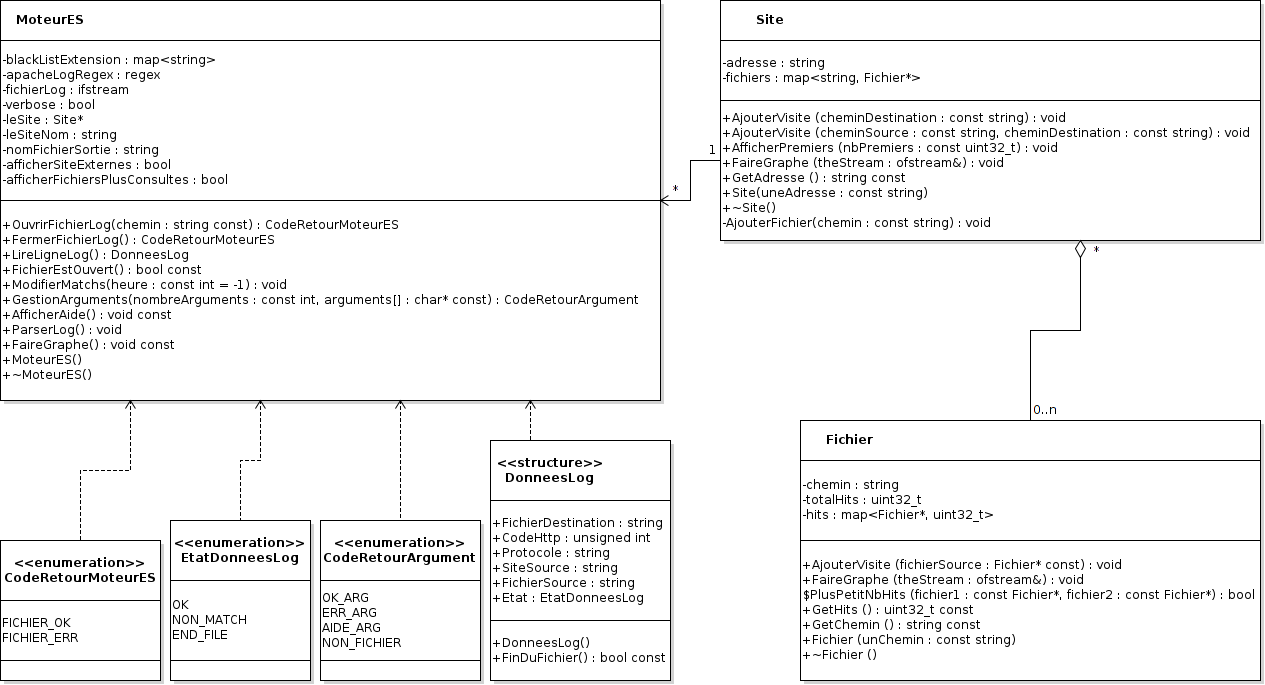
\includegraphics[height=13cm,keepaspectratio]{uml.png}
\caption{Diagramme de classes de l'application}
\label{fig:my_label}
\end{figure}
\end{landscape}
\restoregeometry
\end{document}
